\documentclass[fleqn, 11pt]{article}

\usepackage{verbatim}
\usepackage{amsmath}
\DeclareMathOperator*{\argmin}{arg\,min}
\usepackage{amssymb}
\usepackage{amsthm}
\usepackage{hyperref}
\usepackage{ulem}
\usepackage{enumitem}
\usepackage[top=1.0in, left=0.75in, right=0.75in, bottom=0.75in]{geometry}
\usepackage{graphicx}

\setlength{\headheight}{15pt}

\usepackage{import}

\usepackage{setspace}

\newcommand{\bs}[1]{\boldsymbol{#1}}
\newcommand\norm[1]{\left\lVert#1\right\rVert}
\newcommand{\R}[0]{\mathbb{R}}
\newcommand{\HRule}{\rule{\linewidth}{0.5mm}} 

\usepackage{array}
\usepackage{caption}
\usepackage{floatrow}
\usepackage{multirow}

\usepackage{chngcntr}
\counterwithin*{equation}{section}
\counterwithin*{equation}{subsection}

\usepackage{sectsty}
\sectionfont{\centering}

\usepackage[perpage]{footmisc}

\usepackage{fancyhdr}
\pagestyle{fancy}
\fancyhf{}
\lhead{190100036 \& 190100044}
\rhead{CS 754: Assignment 4}
\renewcommand{\footrulewidth}{1.0pt}
\cfoot{Page \thepage}

\setlength{\parindent}{0em}
\renewcommand{\arraystretch}{2}%

\title{Assignment 4: CS 754}
\author{ 
\begin{tabular}{|c|c|}
     \hline
     \textsf{Krushnakant Bhattad} & \textsf{Devansh Jain} \\
     \hline
     \textsf{190100036} & \textsf{190100044}\\
     \hline
\end{tabular}
}
\date{April 5, 2021}

\begin{document}

\maketitle
\tableofcontents
\thispagestyle{empty}
\setcounter{page}{0}

\newpage
\section*{Question 1}
\addcontentsline{toc}{section}{Question 1}
\setcounter{equation}{0}

\subsection*{Instructions for running the code:}
\begin{itemize}[noitemsep]
    \item After extracting submitted file, look for a directory named \texttt{q1}, and \texttt{cd} (change directory) to it.
    \item Run the file \texttt{q1.m}.
    \item The plots can be found in \texttt{./plots/}.
\end{itemize}

\bigskip

\subsection*{Choosing Dictionary and CS-solvers parameters}
We know that $\bs{f_1}$ is sparse in DCT basis and $\bs{f_2}$ is sparse in Time domain. \\
However $\bs{f} = \bs{f_1} + \bs{f_2}$ is sparse in neither DCT basis nor Time domain. \\
So, we create a over-complete dictionary $\bs{A}$ by concatenating DCT basis and Identity basis (matrix). \\
$\bs{f}$ is sparsely representable in $\bs{A}$.\\

The OMP implementation provided by Prof. Rajwade as part of Assignment 1 solution (matches with our implementation for Assignment 1 but with additional checks) was used (present in \texttt{omp\_error.m}). \\
The parameters to the function are $\bs{A}$, $\bs{f}$ and $\sigma$. \\
Line 4 in \texttt{omp\_error.m} uses $\sigma$ to calculate error bound $e = n \sigma^2$. \\

\bigskip

\subsection*{Explaining Code}
\subsubsection*{Creating the Over-complete Dictionary}
\begin{verbatim}
% DCT matrix
dctmat = dctmtx(256);
% Over-complete dictionary for cosine + spikes
A = [dctmat eye(256)];
\end{verbatim}

\subsubsection*{Generating $\bs{f}$}
Here, \texttt{s} is the sparsity level of $\bs{f_1}$ and $\bs{f_2}$.
\begin{verbatim}
ind1 = randi(256, s, 1);
coeff1 = zeros(256,1);
coeff1(ind1) = rand(s,1)*100;
ind2 = randi(256, s, 1);
coeff2 = zeros(256,1);
coeff2(ind2) = rand(s,1)*100;

f1 = dctmat*coeff1;
f2 = coeff2;
f = f1 + f2;

sigma = 0.01 * abs(mean(f));
f = f + randn(256,1)*sigma;
\end{verbatim}

\subsubsection*{Reconstruction of $\bs{f_1}$ and $\bs{f_2}$}
\begin{verbatim}
x = omp_error(A, f, sigma);
coeff1_recon = x(1:256);
coeff2_recon = x(257:512);

f1_recon = dctmat*coeff1_recon;
f2_recon = coeff2_recon;
\end{verbatim}

\bigskip

\subsection*{Varying $\sigma$ and fixed sparsity level $s$}
\subsubsection*{Plots:}
\begin{figure}[H]
    \centering
    \begin{floatrow}
      \ffigbox[\FBwidth]
      {\caption{Reconstruction Error in $\bs{f_1}$}}
      {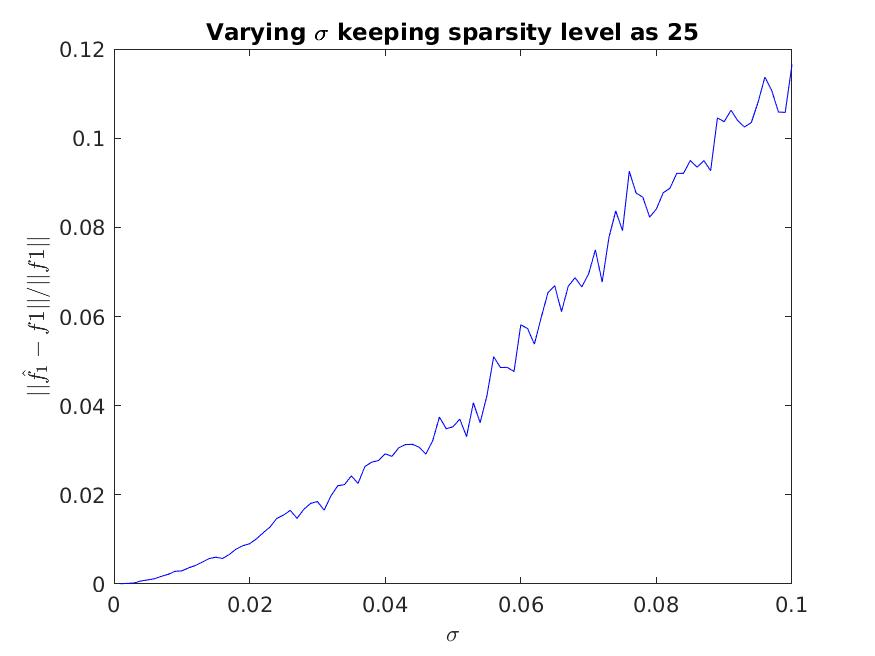
\includegraphics[scale=0.3]{error1_sigma.jpg}}
      
      \ffigbox[\FBwidth]
      {\caption{Reconstruction Error in $\bs{f_2}$}}
      {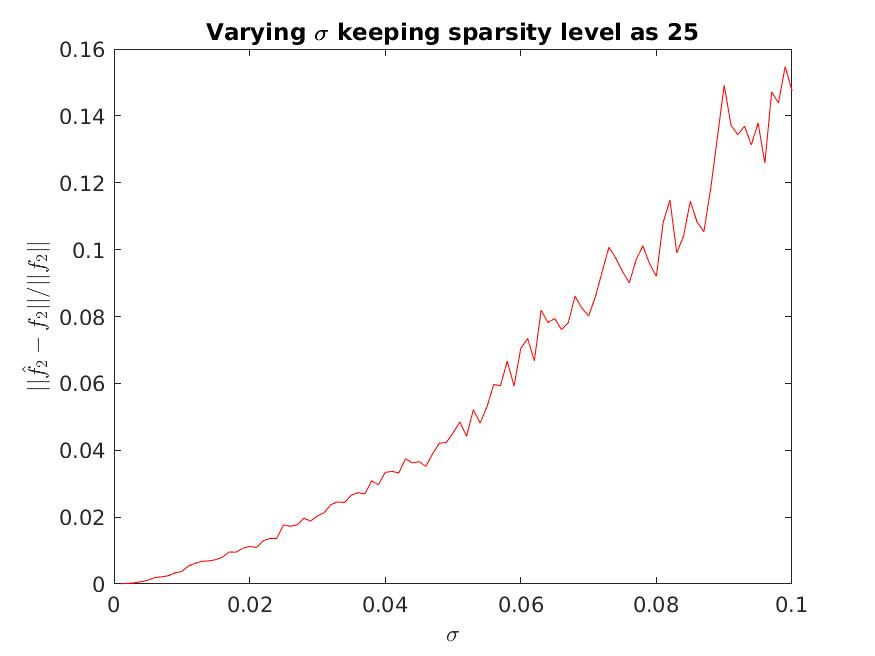
\includegraphics[scale=0.3]{error2_sigma.jpg}}
    \end{floatrow}
\end{figure}

\subsubsection*{Comments:}
\begin{itemize}
    \item $\sigma$ ranges from 0.001 to 0.1 $\times$ (average value of $\bs{f_1} + \bs{f_2}$).
    \item We can clearly see increase in reconstruction error for both $\bs{f_1}$ and $\bs{f_2}$ as $\sigma$ increases.
\end{itemize}

\subsection*{Varying sparsity level $s$ with fixed $\sigma$}
\subsubsection*{Plots:}
\begin{figure}[H]
    \centering
    \begin{floatrow}
      \ffigbox[\FBwidth]
      {\caption{Reconstruction Error in $\bs{f_1}$}}
      {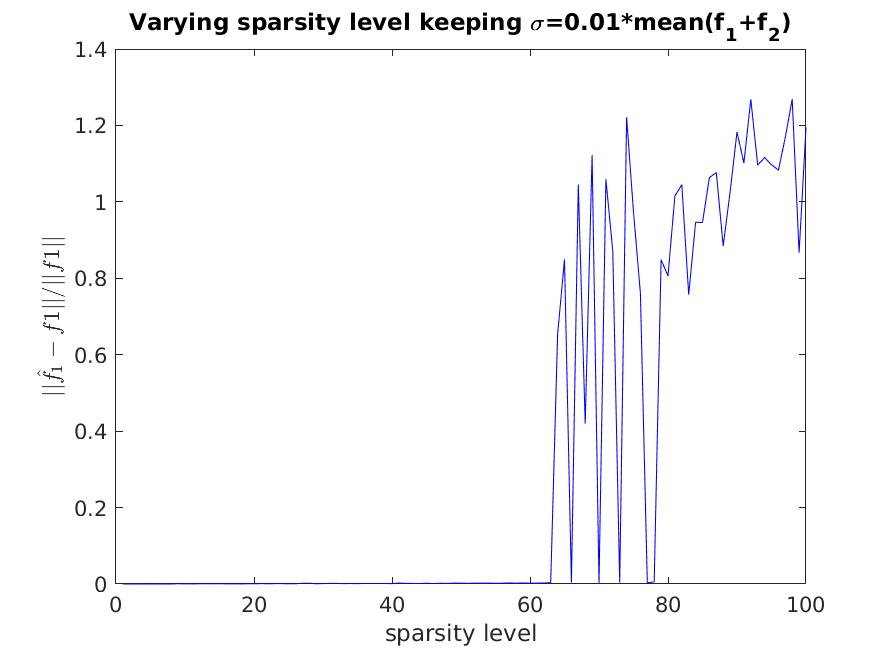
\includegraphics[scale=0.3]{error1_sparsity.jpg}}
      
      \ffigbox[\FBwidth]
      {\caption{Reconstruction Error in $\bs{f_2}$}}
      {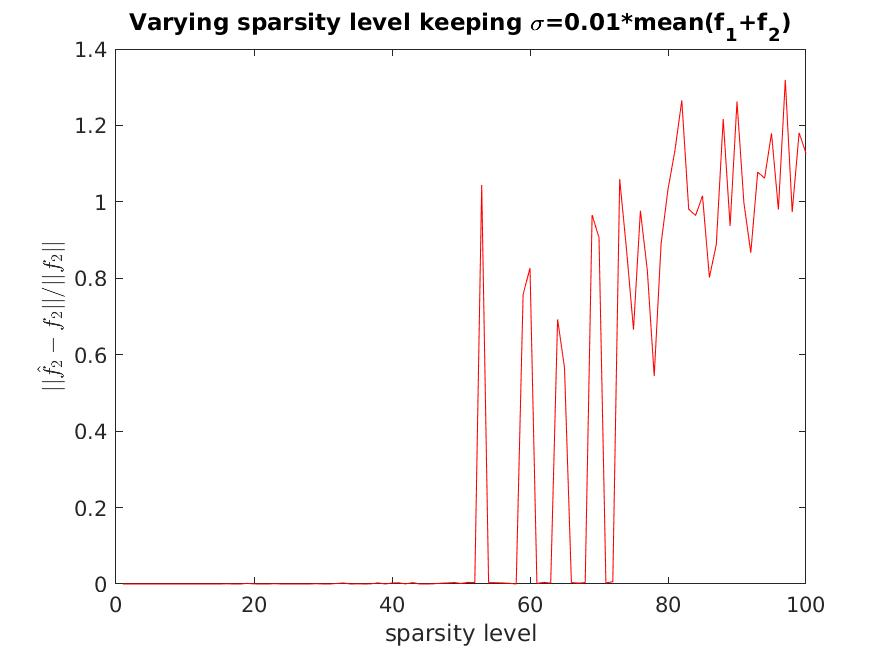
\includegraphics[scale=0.3]{error2_sparsity.jpg}}
    \end{floatrow}
\end{figure}

\subsubsection*{Comments:}
\begin{itemize}
    \item Sparsity level $s$ ranges from 1 to 100.
    \item Reconstruction error is negligible/acceptable till around sparsity level of about 64 (25\% of N=256). \\
    We see a sudden rise in error reaching 1 by sparsity level of 70.
    \item If we zoom into the first part of the plot, we will see a very slow rise (not consistent but visible) in reconstruction error for both $\bs{f_1}$ and $\bs{f_2}$ with increase in sparsity level $s$.
\end{itemize}

\subsection*{Varying magnitude ratio $k$}
\subsubsection*{Plots:}
\begin{figure}[H]
    \centering
    \begin{floatrow}
      \ffigbox[\FBwidth]
      {\caption{Reconstruction Error in $\bs{f_1}$}}
      {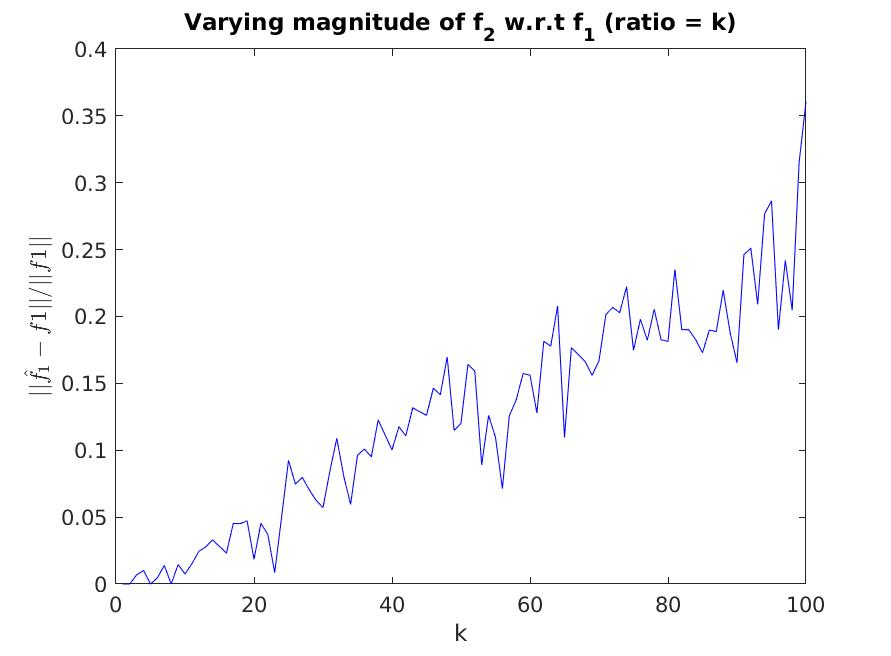
\includegraphics[scale=0.3]{error1_k.jpg}}
      
      \ffigbox[\FBwidth]
      {\caption{Reconstruction Error in $\bs{f_2}$}}
      {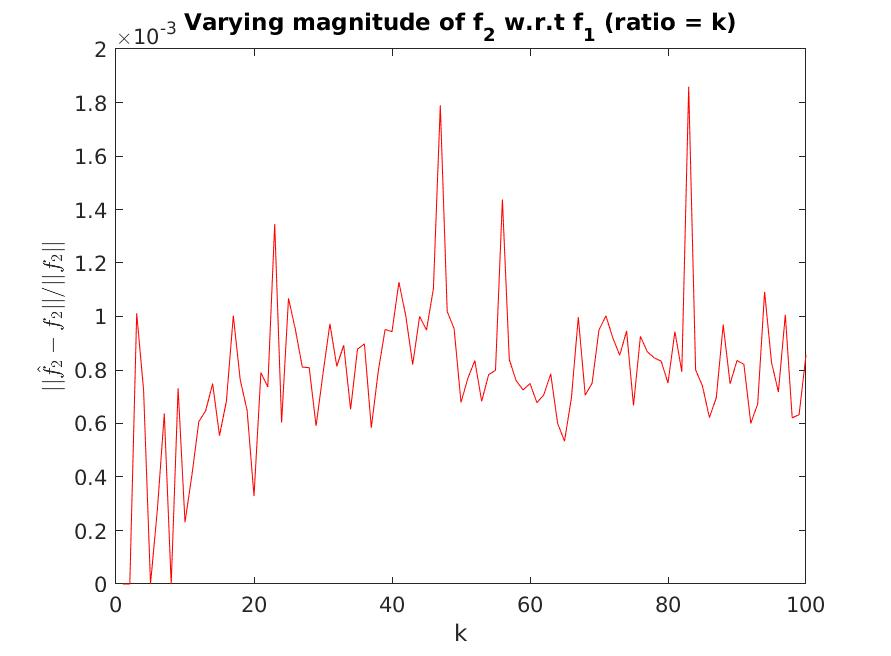
\includegraphics[scale=0.3]{error2_k.jpg}}
    \end{floatrow}
\end{figure}

\subsubsection*{Comments:}
\begin{itemize}
    \item The magnitude of $\bs{f_2}$ is $k$ times that of $\bs{f_1}$
    \item We can clearly see increase in reconstruction error for both $\bs{f_1}$ as $k$ increases. \\
    However, the reconstruction error for $\bs{f_2}$ is almost consistent at around 0.001.
    \item The possible explanation of this could be the decrease in significance of $\bs{f_1}$ in $\bs{f}$, so the error bound in OMP exits when the error value of $\bs{f_2}$ is less as error value of $\bs{f_1}$ becomes less significant with increase in $k$.
    \item To add to that, $\sigma$ is based on the average value of $\bs{f_1} + \bs{f_2}$, which increases while the average value of $\bs{f_1}$ remains same, thus giving similar results as the experiment when we were varying $\sigma$. \\
    For $\bs{f_2}$, increase in $\sigma$ is counter-acted by the increase in average value of $\bs{f_2}$, thus giving us almost consistent reconstruction error.
\end{itemize}


\newpage
\section*{Question 2}
\addcontentsline{toc}{section}{Question 2}
\setcounter{equation}{0}


\textbf{Question: }

\smallskip
We have studied two greedy algorithms for compressive recovery in class - MP and OMP.

\smallskip

Find out a research paper that proposes a greedy algorithm for CS recovery that is
different from OMP and MP. Write down the algorithm in your report, state the key theorem and explain the
meaning of the terms involved.

\vspace{10pt}

\begin{spacing}{0.05}
\noindent
\HRule\\
\HRule
\end{spacing}

\vspace{10pt}

\medskip

\textbf{\large Answer: }

\medskip

There are various greedy algorithms that focus on solving the central problem in CS Recovery, \\
The Basis Pursuit problem: $\min \norm{\bs{x}}_{\ell_1} $ subject to $\bs{y = \Phi x}$. 
Here, we'll describe one such algorithm.

\medskip

\textbf{The Algorithm}: Subspace Pursuit 

\medskip

\textbf{Paper Title}: Subspace Pursuit for Compressive Sensing Signal
Reconstruction

\medskip

\textbf{Paper by}: Wei Dai and Olgica Milenkovic, 
Department of Electrical and Computer Engineering, UIUC

\medskip

\textbf{Link to the paper}: \url{http://arXiv.org/abs/0803.0811v3}

\hrulefill

\subsection*{Introduction}

The main contribution of this paper is a new algorithm,
termed the subspace pursuit (SP) algorithm. It has provable
reconstruction capability comparable to that of LP methods,
and exhibits the low reconstruction complexity of matching
pursuit techniques for very sparse signals. The algorithm can
operate both in the noiseless and noisy regime, allowing
for exact and approximate signal recovery, respectively.
The basic idea behind the SP algorithm is borrowed from
coding theory, more precisely, the $A*$ order-statistic algorithm  
for additive white Gaussian noise channels.

\hrulefill

\subsection*{Some Definitions}

(Note: $\Phi^*$ denotes the transpose of the real valued matrix $\Phi$)

\medskip


\textbf{1. \textit{Truncation} and \textit{span} }: 

\smallskip

Let $\bs{\Phi} \in \R^{m \times N}$, $\bs{x} \in \R^N$ and $I \subset \{ 1,2,..., N \} $ 

\smallskip

$\bs{\Phi}_{I}$ denotes the matrix consisting of the columns $\bs{\Phi}$ of with indices $i \in I$. 

\smallskip

$\bs{x}_{I}$ is composed of the entries of $\bs{x}$
indexed by $i \in I$. 

\smallskip

$span(\bs{\Phi}_{I})$ denotes the space spanned by the columns of the matrix $\bs{\Phi}_{I}$.


\bigskip 

\textbf{2. \textit{Projection} and \textit{Residue} }: 

\smallskip

Let $\bs{y} \in \R^m$ and $\bs{\Phi} \in \R^{m \times n}$. 

Suppose  $\bs{\Phi^*\Phi}$ is invertible. 

Then, the projection of $\bs{y}$ onto  $span(\bs{\Phi})$ is defined as:
\begin{center}
    $\bs{y}_p = proj( \bs{y} ,\bs{\Phi}  )  = \bs{\Phi \Phi^{\dagger} y }  $ 
\end{center}

Here, $\dagger$ denotes psuedo-inverse: $\Phi^{\dagger} = \bs{(\Phi^*\Phi)^{-1}\Phi^*}  $

\medskip

The residue vector of the projection is: 
\begin{center}
    $\bs{y}_r = resid( \bs{y} ,\bs{\Phi}  )  = \bs{y - y_p } $ 
\end{center}


\newpage 


\subsection*{The Psuedo-Code of the SP Algorithm}

\medskip

\textbf{\textit{Input}}: $K, \bs{\Phi}, \bs{y}$

\medskip

\textbf{\textit{Initialisation}}:
\begin{enumerate}
    \item $T^0 = $ \{ $K$ indices corresponding to the largest magnitude entries in the vector $\bs{\Phi^*y}$ \} 
    \item $\bs{y^0_r}  = resid ( \bs{y}, \bs{\Phi}_{T^0} ) $
\end{enumerate}

\textbf{\textit{Iteration}}:
At the $i^th$ iteration, do:

\begin{enumerate}
    \item $\Tilde{T^l} = T^{l-1} \cup $ \{ $K$ indices corresponding to the largest magnitude entries in the vector $\bs{\Phi^*y^{i-1}_r}$ \}
    \item Set $\bs{x}_p = \bs{\Phi}^{\dagger}_{T^i}  $
    \item $T^i = $ \{ $K$ indices corresponding to the largest magnitude entries in the vector $\bs{x}_p$ \} 
    \item $\bs{y^i_r}  = resid ( \bs{y}, \bs{\Phi}_{T^i} ) $
    \item If $\norm{\bs{y^i_r}  }_2 > \bs{y^{i-1}_r}  $,  let ${T^i}= {T^{i-1}}$ and quit the iteration
\end{enumerate} 

\textbf{\textit{Output}}:

Let $\bs{x}_{T^i} = \bs{\Phi}^{\dagger}_{T^i}  $, and set all other entries to 0. Output this estimated signal $\bs{x}$.

\hrulefill

\subsection*{Flow Chart}

The following Flow Chart can assist in better understanding of the algorithm: 

\includegraphics[scale=0.34]{SP_Flowchart.png}

It is directly taken from the paper, but it does help a great deal in  understanding of the algorithm.

\newpage

\subsection*{Performace Bound Theorems }

\medskip

\textbf{Non-Noisy Case: Theorem 1 }

\smallskip

Let $\bs{x} \in \R^k$ be a K-sparse signal, and let
its corresponding measurement be $\bs{y = \Phi x} \in \R^m$ .

\smallskip

If the sampling matrix $\bs{\Phi}$  satisfies the RIP with constant  $\delta_{3K} < 0.165$, then the SP algorithm is guaranteed to \textbf{exactly} recover x from
y via a finite number of iterations.

\smallskip


Since this is an exact recovery, ``bounds" are not needed. 


\hrulefill

\medskip

\textbf{Noisy Case: Theorem 9 }

\smallskip

Let $\bs{x} \in \R^k$ be a K-sparse signal, and let
its corresponding measurement be $\bs{y = \Phi x + e}  \in \R^m$, 

where $\bs{e}$  denotes the noise vector. 

\smallskip

Suppose that the sampling matrix satisfies
the RIP with parameter $\delta_{3K} < 0.083 $.  

\smallskip

Then the reconstruction distortion of the SP algorithm satisfies
\begin{center}
    $\norm{\bs{x - \hat{x}}}_2 \leq c_K \norm{\bs{e}}_2$
\end{center}

Here, $\bs{x}$ is the original signal, and $\bs{\hat{x}}$ is the estimated signal. 

\smallskip

Also, $c_K$ is a constant independent of $\bs{x}$, equal to $\dfrac{1+\delta_{3K}+\delta_{3K}^2}{\delta_{3K}(1-\delta_{3K})}$

\smallskip

\hrulefill

\medskip


\textbf{Approximate Case: Theorem 9, Corollary 1} 

\smallskip

Let $\bs{x} \in \R^k$ be an approximately K-sparse signal, and let
its corresponding measurement be 

$\bs{y = \Phi x + e}  \in \R^m$, where $\bs{e}$  denotes the noise vector.

\smallskip

Suppose that the sampling matrix satisfies
the RIP with parameter $\delta_{6K} < 0.083 $.  

\smallskip

Then the reconstruction distortion of the SP algorithm satisfies
\begin{center}
    $\norm{\bs{x - \hat{x}}}_2 \leq c_{2K} (\norm{\bs{e}}_2 + c^{'}_{K}  ) \norm{\bs{x - x_K}}_1 $
\end{center}

Repeating notations are same. $\bs{x_K}$ is the the vector obtained from $\bs{x}$ by maintaining the
K entries with largest magnitude and setting all other entries
in the vector to zero.

\smallskip

$c^{'}_{K}$ is a constant independent of $\bs{x}$, equal to $\sqrt{\dfrac{1+\delta_{6K}}{K}}$

\hrulefill

\newpage
\section*{Question 3}
\addcontentsline{toc}{section}{Question 3}
\setcounter{equation}{0}

\textbf{Given:} \\
Dictionary $\bs{D}$ contains images $\bs{d_k} \ (k \in \{1, \dots, M\})$, each of same dimension as images of class $\mathcal{S}$. \\
All images $\bs{s_i}$ in class $\mathcal{S}$ are sparsely represented in dictionary $\bs{D}$, i.e., $\bs{s_i} = \sum_{k=1}^{M} \alpha_k \bs{d_k}$ where $\{\alpha_k\}_{k=1}^{k=M}$ is a sparse vector. \\

\medskip

\subsection*{(a)}
Class $\mathcal{S}_1$ which consists of images obtained by applying a known derivative filter to the images in $\mathcal{S}$. \\
Image $\bs{x_i}$ in Class $\mathcal{S}_1$ is obtained by applying a known derivative filter $\bs{d}$ to the image $\bs{s_i}$ in $\mathcal{S}$.

\begin{equation*}
    \begin{aligned}
        \bs{x_i} &= \bs{d} \bs{*} \bs{s_i} \\
            &= \bs{d} \bs{*} \sum_{k=1}^{M} \alpha_k \bs{d_k} \\
            &= \sum_{k=1}^{M} \alpha_k (\bs{d} \bs{*} \bs{d_k}) \ \ (\text{Distributive Property of Convolution)}\\
    \end{aligned}
\end{equation*}

As we know that $\{\alpha_k\}_{k=1}^{k=M}$ is a sparse vector. \\
All images $\bs{x_i}$ in class $\mathcal{S}_1$ are sparsely represented in dictionary $\bs{D_1} = \{\bs{d} \bs{*} \bs{d_k} | \bs{d_k} \in \bs{D}\}$. \\

\medskip

\subsection*{(b)}
Class $\mathcal{S}_2$ which consists of images obtained by rotating a subset of the images in class $\mathcal{S}$ by a known fixed angle $\alpha$, and the other subset by another known fixed angle $\beta$. \\
Rotating of an image by angle $\theta$ is equivalent to pre-multiplying original with a matrix $\bs{A_\theta}$\footnote{refer to comments at the end of question for construction}.

\begin{equation*}
    \begin{aligned}
        \bs{x_i} &= \bs{A_\theta} \bs{s_i} \\
            &= \bs{A_\theta} \sum_{k=1}^{M} \alpha_k \bs{d_k} \\
            &= \sum_{k=1}^{M} \alpha_k (\bs{A_\theta} \bs{d_k}) \\
    \end{aligned}
\end{equation*}

As we know that $\{\alpha_k\}_{k=1}^{k=M}$ is a sparse vector. \\
Image $\bs{x_i}$ in Class $\mathcal{S}_2$ is obtained by rotating the image $\bs{s_i}$ in $\mathcal{S}$ by either $\alpha$ or $\beta$, it can be represented as sparse linear combination of $\bs{A_\alpha} \bs{d_k}$ or $\bs{A_\beta} \bs{d_k}$. \\
All images $\bs{x_i}$ in class $\mathcal{S}_2$ are sparsely represented in dictionary $\bs{D_2} = \{\bs{A_\alpha} \bs{d_k} | \bs{d_k} \in \bs{D}\} \cup \{\bs{A_\beta} \bs{d_k} | \bs{d_k} \in \bs{D}\}$. \\

\newpage

\subsection*{(c)}
Class $\mathcal{S}_3$ which consists of images obtained by applying an intensity transformation $I^i_{new}(x,y) = \alpha (I^i_{old}(x,y))^2 + \beta (I^i_{old}(x,y)) + \gamma$ to the images in $\mathcal{S}$, where $\alpha,\beta,\gamma$ are known. \\
Image $\bs{x_i}$ in Class $\mathcal{S}_3$ is obtained by by applying an intensity transformation to $\bs{s_i}$ in $\mathcal{S}$.

\begin{equation*}
    \begin{aligned}
        \bs{s_i}(x, y) &= \sum_{k=1}^{M} \alpha_k \bs{d_k}(x,y) \ \ (\Longleftrightarrow \bs{s_i} = \sum_{k=1}^{M} \alpha_k \bs{d_k}) \\
        \bs{x_i}(x, y) &= \alpha(\bs{s_i}(x, y))^2 + \beta(\bs{s_i}(x, y)) + \gamma \\
            &= \alpha(\sum_{k=1}^{M} \alpha_k \bs{d_k}(x,y))^2 + \beta(\sum_{k=1}^{M} \alpha_k \bs{d_k}(x,y)) + (\gamma) \\
            &= (\sum_{k=1}^{M} \alpha \alpha_k^2 (\bs{d_k}(x,y))^2) + (\sum_{k=1}^{M} \sum_{l>k}^{M} \alpha \alpha_k \alpha_l (\bs{d_k}(x,y))(\bs{d_l}(x,y))) + (\sum_{k=1}^{M} \beta \alpha_k (\bs{d_k}(x,y))) + (\gamma (\bs{1})) \\
            &(\Longleftrightarrow \bs{x_i} = (\sum_{k=1}^{M} \alpha \alpha_k^2 (\bs{d_k}.\wedge2)) + (\sum_{k=1}^{M} \sum_{l>k}^{M} \alpha \alpha_k \alpha_l (\bs{d_k}.*\bs{d_l})) + (\sum_{k=1}^{M} \beta \alpha_k \bs{d_k}) + (\gamma \bs{1}) \\
    \end{aligned}
\end{equation*}

As we know that $\{\alpha_k\}_{k=1}^{k=M}$ is a sparse vector, $\{\alpha \alpha_k^2\}_{k=1}^{k=M} \cup \{\alpha \alpha_k \alpha_l\}_{k=1,l>k}^{k=M,l=M} \cup \{\beta \alpha_k\}_{k=1}^{k=M} \cup \{\gamma\}$ is also a sparse vector (percentage sparsity doesn't increase). \\
All images $\bs{x_i}$ in class $\mathcal{S}_3$ are sparsely represented in dictionary $\bs{D_3} = \bs{D} \cup \{\bs{1}, \text{vector contains all 1s}\} \cup \{\bs{d_k}.\wedge2 | \bs{d_k} \in \bs{D}\} \cup \{\bs{d_k}.*\bs{d_l} | \bs{d_k}, \bs{d_l} \in \bs{D}, l > k\}$. \\

\medskip

\subsection*{(d)}
Class $\mathcal{S}_4$ which consists of images obtained by applying a known blur kernel to the images in $\mathcal{S}$. \\
Image $\bs{x_i}$ in Class $\mathcal{S}_4$ is obtained by applying a known blur kernel $\bs{\omega}$ to the image $\bs{s_i}$ in $\mathcal{S}$.

\begin{equation*}
    \begin{aligned}
        \bs{x_i} &= \bs{\omega} \bs{*} \bs{s_i} \\
            &= \bs{\omega} \bs{*} \sum_{k=1}^{M} \alpha_k \bs{d_k} \\
            &= \sum_{k=1}^{M} \alpha_k (\bs{\omega} \bs{*} \bs{d_k}) \ \ (\text{Distributive Property of Convolution)}\\
    \end{aligned}
\end{equation*}

As we know that $\{\alpha_k\}_{k=1}^{k=M}$ is a sparse vector. \\
All images $\bs{x_i}$ in class $\mathcal{S}_4$ are sparsely represented in dictionary $\bs{D_4} = \{\bs{\omega} \bs{*} \bs{d_k} | \bs{d_k} \in \bs{D}\}$. \\

\medskip

\subsection*{(e)}
Class $\mathcal{S}_5$ which consists of images obtained by applying a blur kernel which is known to be a linear combination of blur kernels belonging to a known set $\mathcal{B}$, to the images in $\mathcal{S}$. \\
Image $\bs{x_i}$ in Class $\mathcal{S}_5$ is obtained by applying a blur kernel $\bs{\omega}$ which is known to be a linear combination\footnote{I have assumed that we don't know this linear combination and it may vary for different $\bs{x_i}$s.} of blur kernels belonging to a known set $\mathcal{B}$, to the image $\bs{s_i}$ in $\mathcal{S}$.

\begin{equation*}
    \begin{aligned}
        \bs{\omega} &= \sum_{j=1}^{b} \beta_j \bs{b_j} \ \  (\bs{b_j} \in \mathcal{B}) \\
        \bs{x_i} &= \bs{\omega} \bs{*} \bs{s_i} \\
            &= \bs{\omega} \bs{*} \sum_{k=1}^{M} \alpha_k \bs{d_k} \\
            &= \sum_{k=1}^{M} \alpha_k (\bs{\omega} \bs{*} \bs{d_k}) &\ \ (\text{Distributive Property of Convolution)}\\
            &= \sum_{k=1}^{M} \alpha_k ((\sum_{j=1}^{b} \beta_j \bs{b_j}) \bs{*} \bs{d_k}) \\
            &= \sum_{k=1}^{M} \alpha_k (\sum_{j=1}^{b} \beta_j (\bs{b_j} \bs{*} \bs{d_k})) &\ \ (\text{Distributive Property of Convolution)}\\
            &= \sum_{k=1}^{M} \sum_{j=1}^{b} \alpha_k \beta_j (\bs{b_j} \bs{*} \bs{d_k}) \\
    \end{aligned}
\end{equation*}

As we know that $\{\alpha_k\}_{k=1}^{k=M}$ is a sparse vector, $\{\alpha_k \beta_j\}_{k=1, j=1}^{k=M, j=b}$ is also a sparse vector (percentage sparsity doesn't increase). \\
All images $\bs{x_i}$ in class $\mathcal{S}_5$ are sparsely represented in dictionary $\bs{D_5} = \{\bs{b_j} \bs{*} \bs{d_k} | \bs{d_k} \in \bs{D}, \bs{b_j} \in \mathcal{B} \}$. \\ Dictionary contains $Mb$ images.

\subsection*{Comments:}
\begin{itemize}
    \item Distributive Property of Convolution has been used in (a), (d) and (e). \\ Reference: \url{http://ccc.inaoep.mx/~a.morales/DSP/pdf/DSP_4_convolution_prop.pdf}, page 36.
    \item In (c) and (e), number of atoms present in the dictionary has increased significantly, however, percentage sparsity is maintained (in fact, decreased in (c)).
    \item Derivative filter uses convolution, so does blur kernel, so the results are similar. \\
    Reference: \url{https://en.wikipedia.org/wiki/Image_derivatives} (Derivative Filter), \\ \url{https://en.wikipedia.org/wiki/Kernel_(image_processing)} (Blue Kernel)
    \item Construction of $\bs{A_\theta}$ used in (b), can be complex and depends on how the image is rotated. \\
    Several methods are stated here, \url{https://datagenetics.com/blog/august32013/index.html}. \\
    In all cases, pixel value in rotated image is some linear combination of original value, this can be represented as a matrix $\bs{A_\theta}$ of size $n^2 \times n^2$. \\
    Padding and/or cropping can make the transformation formula more complex. \\
    In simplest case, $\bs{x_i}(x, y) = \bs{s_i}(x \cos{\theta} + y \sin{\theta}, -x \sin{\theta} + y \cos{\theta})$ if $(x \cos{\theta} + y \sin{\theta}, -x \sin{\theta} + y \cos{\theta})$ lies in region else $0$.
\end{itemize}


\newpage
\section*{Question 4}
\addcontentsline{toc}{section}{Question 4}
\setcounter{equation}{0}

\subsection*{Part (1)}

\textbf{Question: }

\smallskip

$\bs{A}$, a $m \times n$ matrix of rank greater than $r$ , is known apriori.

\smallskip

We seek to minimize $J(\bs{Q})$:
\begin{center}
    $J(\bs{Q}) = \|\bs{A}-\bs{Q}\|^2_F$, where $\bs{Q}$ is a rank-$r$ matrix, with $r < m, \; r < n$
\end{center}
\hrulefill

\medskip

\textbf{Answer: }

\medskip

The arg min of $J(\bs{Q})$ is $\bs{A_r=U \Sigma_r V^T}$ 

\smallskip

where $\bs{U \Sigma V^T}$ is the singular value decomposition of $\bs{A}$ \\
$\bs{\Sigma_r} $ is same as the matrix
$\bs{\Sigma} $, with all but the top $r$ Singular values in $\bs{\Sigma}$ taken as 0.

\hrulefill

\medskip

\textbf{Justification: }

A proof of the result above is here: \url{https://link.springer.com/article/10.1007\%2FBF02288367}. \\
Here, we provide another argument.

\medskip

For a matrix $M$ let $\sigma_i(M)$ denote the $i^{\text{th}}$ largest singular value.
WLOG assume $n \geq  m$.
Then, we have the following: 

\textit{Lemma: } For $m \times n$ matrices $X,Y$ with $q \leq i, j \leq n$, 
we have
\begin{center}
   $ \sigma_{i+j - 1}(X + Y) \leq \sigma_i(X) + \sigma_j(Y) $
\end{center}

It is one of Weyl's inequalities. 

A proof can be found here: \url{https://qchu.wordpress.com/2017/03/13/singular-value-decomposition/}, 
under the section "Additive perturbation (Weyl)". 

In this inequality, substitute $X = A-B, Y = B, j = r+1$ to get:
\begin{center}
    $\sigma_{i+r}(A) \leq \sigma _{i}(A - B) + \sigma_{r+1}(B)$
\end{center}
Thus, we have,
    \begin{align*}
\|A - B\|_F^2 &= 
\sum_{i=1}^n \sigma_i^2(A - B) \geq 
\sum_{i=1}^{n-r} \sigma_i^2(A - B)
\\ & \geq \sum_{i=r+1}^{n} \sigma_i^2(A)
\end{align*}
And equality is attained when we set $B=A_r$ as defined earlier. 


\hrulefill

\subsection*{An Intuitive Argument: }


\medskip

Suppose $\bs{A}$ has rank-$p$.

Let $\bs{U \Sigma V^T}= \displaystyle \sum_{i=1}^{p} \sigma_i \bs{u_i v_i^T}  $ be the singular value decomposition of $\bs{A}$. 


For $\bs{N}$,  a $n \times d$ matrix : think of the rows of  $\bs{N}$ as n points in d-dimensional
space. The Frobenius norm of  $\bs{N}$ is the square root of the sum of the squared distance of
the points to the origin. We will use this interpretation in this problem. 

\newpage

{ \large  \textbf{\textit{Claim 4.1.1:}}} Interpretation of $\bs{A_r}$

\medskip

The rows of $\bs{A_r}$ are the projections of the rows of $\bs{A}$ onto the subspace $\bs{V_r}$
spanned by the first $r$ right singular vectors of $\bs{A}$. 


{\textit{Proof: }} Let $a$ be an arbitrary row vector.

Since the $\bs{v_i}$ are orthonormal, the projection of the vector $a$ onto $\bs{V_r}$ is given by 
$\displaystyle \sum_{i=1}^{r} (a \cdot \bs{v_i}) \bs{v_i}^T $

Thus, the matrix whose rows are the
projections of the rows of $\bs{A}$ onto $\bs{V_r}$  is given by 
$\displaystyle \sum_{i=1}^{r} \bs{A} \bs{v_i} \bs{v_i}^T $

This last expression simplifies to $\displaystyle \sum_{i=1}^{r} \bs{A} \bs{v_i} \bs{v_i}^T =  \displaystyle \sum_{i=1}^{r} \sigma_i \bs{u_i v_i^T} = \bs{A_r}  $


Thus the claim is proved. 

\bigskip 

{ \large  \textbf{\textit{Claim 4.1.2:}}} For any matrix $B$ of rank at most $r$, 
$  \|\bs{A}-\bs{A_r}\|^2_F \leq \|\bs{A}-\bs{B}\|^2_F $

\medskip 

Let $\bs{B}$ minimize $ \|\bs{A}-\bs{B}\|^2_F$ among all rank $r$ or less matrices.

\smallskip

Let $\bs{V}$ be the space
spanned by the rows of $\bs{B}$. The dimension of $\bs{V}$  is at most k.  

\medskip

Since  $\bs{B}$ minimizes $ \|\bs{A}-\bs{B}\|^2_F$, it must be that each row of $\bs{B}$ is the projection of the corresponding row of $\bs{A}$ onto $\bs{V}$, otherwise replacing the row of $\bs{B}$ with the projection of the corresponding row of $\bs{A}$ onto $\bs{V}$
does not change $\bs{V}$ and hence the rank of $\bs{B}$ but would reduce $ \|\bs{A}-\bs{B}\|^2_F$

\smallskip

Since each row
of $\bs{B}$ is the projection of the corresponding row of $\bs{A}$, it follows that $ \|\bs{A}-\bs{B}\|^2_F$ is the sum
of squared distances of rows of  $\bs{A}$  to  $\bs{V}$ .  

\smallskip

Since $\bs{A_r}$   minimizes 
the sum of squared distance
of rows of $\bs{A}$  to any $r$-dimensional subspace, the claim follows. 

\hrulefill

\bigskip 

\textbf{Usage: }

\medskip

The best rank-$r$
approximation has an interesting \textbf{application to image compression}. 

\smallskip

This is based on the fact that, digital images are in fact, stored as matrices; and it is 
empirically observed that these are inherently low rank.

\smallskip

Thus, we store the image matrix as its low(enough) rank approximation instead. 

\smallskip

Suppose $\mathcal{I}$ is an image with values in $\R^{m \times n}$. Then the space needed to store $\mathcal{I}$  
is $\mathcal{O}(m*n)$. We store info about the rank$-r$ approximation of 
$\mathcal{I}$ instead, where $r \ll \min\{m,n\}$. 

\smallskip

We perform the SVD of M, and only store the $r$ largest singular values and vectors:

\begin{center}
    $\mathcal{I}_{m \times n} \approx \bs{U_r \Sigma_r V_r ^T } = \mathcal{I}_r  $
\end{center}

We store $\bs{U_r,  \Sigma_r,  V_r }$ instead of  $\mathcal{I}$. The cost is:

\begin{center}
    Cost of $\bs{U_r}$ +  Cost of $\bs{\Sigma_r}$ +  Cost of $\bs{V_r}$  = Total cost \\
    $mk + k + nk = k (m+n+1)$
\end{center}

This is one magnitude smaller than $\mathcal{O}(m*n)$ when $r \ll \min\{m,n\}$. 

The above compression algorithm is otherwise arbitrary. 
The reason why it works with so promising results, is because of  
the particular solution to the optimization problem we solved before.



\newpage

\subsection*{Part (2) }

\textbf{Question: }

\smallskip

Matrices $\bs{A}$ and $\bs{B}$ are both known.

\smallskip

We seek to minimize $J(\bs{R})$ where  $\bs{R}$ is constrained to be orthonormal, and: 
\begin{center}
    $J(\bs{R}) = \|\bs{A}-\bs{R} \bs{B}\|^2_F$, where $\bs{A} \in \mathbb{R}^{n \times m}, \bs{B} \in \mathbb{R}^{n \times m}, \bs{R} \in \mathbb{R}^{n \times n}, m > n$ 

\end{center}
\hrulefill

\medskip

\textbf{Answer: }

\medskip

The arg min of $J(\bs{R})$ with constraint $\bs{R^TR=I}$,  
is $\bs{R=VU^T}$ 

\smallskip

where $\bs{USV^T}$ is the singular value decomposition of $\bs{BA^T}$

\hrulefill

\medskip

\textbf{Justification: }

\medskip


First, we simplify $J(\bs{R})$ as follows: 
\begin{align*}
    J(\bs{R}) &= \|\bs{A}-\bs{R} \bs{B}\|^2_F \\
    &= trace((\bs{A}-\bs{RB})^T (\bs{A}-\bs{RB}))  \\
    &= trace(\bs{A^TA + B^TB -  A^TRB - ( A^TRB  )^T  }) \;\;\;\; \ldots\text{(As $\bs{R^TR=I}$  )}\\
    &= trace(\bs{A^TA + B^TB}) - 2 trace(\bs{A^TRB}) \;\;\;\;\;\;\;\; \;\;\;\; \;\;\; 
    \ldots\text{(As trace($\bs{K^T})=$ trace($\bs{K}$))}\\
\end{align*}

Now, $trace(\bs{A^TA + B^TB})$ is a constant.

Thus to  minimize $J(\bs{R})$ is same as to maximize $trace(\bs{A^TRB})$ under same constraint. 

\medskip 

Further we'll make use of the property that $ trace(AB) = trace(BA) $ 

\smallskip

Thus, firstly, we have $trace(\bs{A^TRB}) = trace(\bs{RBA^T})$

\medskip 

Now suppose the singular value decomposition of $\bs{BA^T}$ is $USV^T$. Then, 
\begin{center}
    $trace(\bs{RBA^T})  =  trace(\bs{RUSV^T}) =  trace(\bs{V^TRUS}) =  trace(\bs{XS}) 
    = \displaystyle \sum_{i=1}^n X_{ii} S_{ii}   $
\end{center}
where, $\bs{X=V^TRU}$ is an orthonormal matrix due to which $|X_{ii}| \leq 1$ 

The singular values $S_{ii}$ are all non-negative, thus the maximum will be obtained when 
for all $i, X_{ii}=1$, i.e. $\bs{X=I}$. 

Thus we need to have $\bs{V^TRU=I}$, that is $\bs{R=VU^T}$


\hrulefill


\newpage 

\textbf{Usage: }

\medskip

The given optimization problem is an important and fundamental problem in various fields, like   \\ 
Computer Vision, Computer Graphics, Medical Imaging (especially in a sub-branch called as `statistical shape analysis') and many more.

\medskip

In image processing specifically, the solution to above optimization problem is required in quite a few places, of which we'll explain one here. 

\medskip 

We'll describe the instance where it is encountered in one of the algorithms in dictionary learning. We use it in the method known as ``\textbf{Union of Orthonormal bases}"

\smallskip

We represent the signal as: $\bs{X}=\bs{AS}+\epsilon$, where $\bs{X} \in \R^{d \times N}$ is the signal, 
$\bs{A} \in \R^{d \times Md} $ is the over-complete dictionary that is a union of ortho-normal
bases,  $\bs{S} \in \R^{Md \times N} $ is 
the sparse co-efficients vector. 

\smallskip

$\bs{A}$ is a the row concatenation of ortho-normal bases $A_i$ for $i \in \{ 1,2,...,M \}$

\smallskip

$\bs{X}$ is a known signal. Assuming we have fixed bases stored in $\bs{A}$, the
coefficients in $\bs{X}$ can be estimated using block
coordinate descent (BCR) . 

\smallskip

Given the coefficients, we next want to update
the dictionary. 

\medskip

For all $m$, we do the following: 
\begin{enumerate}
    \item Get the residual vector: $\bs{ X_m = X} - \displaystyle  \sum_{j \neq m} \bs{A_j S_j }$
    \item Solve for $\bs{A_m}$ as: 
    \begin{center}
            $\bs{A_m} = \argmin_{\bs{A}} \norm{\bs{X_m-AS_m}}^2$ s.t. $\bs{AA^T=A^TA=I}$
    \end{center}
    Here, $\bs{X_m} \in \R^{d \times N}$, $\bs{S_m} \in \R^{d \times N} $ and  $\bs{A} \in \R^{d \times d} $ \\
    It is in this step where we use the minimization problem. 
\end{enumerate}


\newpage


\section*{Question 5}
\addcontentsline{toc}{section}{Question 5}
\setcounter{equation}{0}


\subsection*{Part (a)}

\textbf{Question: }

\smallskip

What is hyperspectral unmixing? 

You may use an equation to support your answer with symbol
meanings carefully explained.

\hrulefill

\medskip

\textbf{Answer: }
\subsubsection*{Meaning of the Terms}

\textbf{\textit{a. Spectral Imaging: }}

\smallskip

Spectral imaging is imaging that uses multiple bands across the electromagnetic spectrum. While an ordinary camera captures light across three wavelength bands in the visible spectrum, red, green, and blue (RGB), spectral imaging encompasses a wide variety of techniques that go beyond RGB. Spectral imaging may use the infrared, the visible spectrum, the ultraviolet, x-rays, or some combination of the above. It may include the acquisition of image data in visible and non-visible bands simultaneously, illumination from outside the visible range, or the use of optical filters to capture a specific spectral range. It is also possible to capture hundreds of wavelength bands for each pixel in an image.

\medskip

\textbf{\textit{b. Hyperspectral Imaging:}}

\smallskip

Hyperspectral imaging, like other spectral imaging, collects and processes information from across the electromagnetic spectrum.[1] The goal of hyperspectral imaging is to obtain the spectrum for each pixel in the image of a scene, with the purpose of finding objects, identifying materials, or detecting processes.

In hyperspectral imaging, a complete spectrum or some spectral information (such as the Doppler shift or Zeeman splitting of a spectral line) is collected at every pixel in an image plane. A hyperspectral camera uses special hardware to capture hundreds of wavelength bands for each pixel, which can be interpreted as a complete spectrum. In other words, the camera has a high spectral resolution.

\medskip

\textbf{\textit{c. Hyperspectral Unmixing:}}

\smallskip

Hyperspectral unmixing is
a procedure that decomposes the measured pixel spectrum
of hyperspectral data into a collection of constituent spectral
signatures (or end-members) and a set of corresponding fractional abundances.

\subsubsection*{Mathematical Formulation}

We focus on a relatively simplistic but very representative
model, known as the Linear Mixing Model(LMM). 

\smallskip

Despite the fact that the LMM is not always true, 
especially under certain scenarios that exhibit strong non-linearity, 
it is generally recognized as an acceptable model 
for many real-world scenarios.

\smallskip

We assume a
macroscopic mixing scale in which the incident light interacts
with only one material before reflecting off.

\medskip

Then, the LMM is described as follows:

\smallskip

Let $y_m[n]$ denote the
hyper-spectral camera’s measurement at spectral band $m$ and at pixel $n$. 

\smallskip

Suppose $M$ is the number of spectral bands, and $L$ is the number of pixels. 

\smallskip

Consider the signal $y[n] = [ y_1[n], y_2[n], \cdots , y_M[n]  ]^T \in \R^M$

\newpage

The LMM is now given by: 

\begin{center}
    $y[n] = \displaystyle \sum_{i=1}^n a_i s_i[n] + v[n] = As[n] + v[n] $.
\end{center}


for $n= 1,2,\ldots, L$,  where:  
\begin{enumerate}
    \item Each $ a_i \in \R^M$ for $i = 1, \ldots, N$ is called an
endmember signature vector which contains the spectral components of a specific material 
(indexed by $i$ ) in the scene

    \item N is the number of endmembers, or materials, in the scene. 

    \item $A = [a_1 \ldots a_N] \in \R^{M \times N}$ is called the endmember matrix. 
    
    \item $s_i[n]$ describes the contribution of material $i$ at pixel $n$.  \\
$s[n] = [ s_1[n] \ldots s_N[n] ] \in \R^N$ is called the abundance vector at
pixel $n$. 

    \item $v[n] \in \R^M $ simply denotes the noise vector at pixel $n$.

\end{enumerate}


Some characteristics of the formulation are:

\begin{itemize}
    \item M is often large— typically more than 200
    \item The mixing process described by the LMM Equation is a consequence of limited spatial resolution of          hyper-spectral cameras. Specifically, one pixel may not be spatially fine enough to contain one material      only.
    \item By nature, the abundance vectors $s[n]$ should satisfy, for every n,  $s_i[n] \geq 0$ and $\sum_{i=1}^n s_i[n]=1$
\end{itemize}

\bigskip

\subsection*{Part (b)}

\textbf{Question: }

\smallskip

In equation 40 of the paper, explain how non-negative matrix factorization is used for hyperspectral unmixing.

\hrulefill

\medskip

\textbf{Answer: }

\smallskip

Treat each $y[n]$ for $n= 1,2,\ldots, L$  as a column vector. 

\smallskip

Then these are column concatened to form $\bs{Y}=[ \; y[1] \; y[2] \; \ldots \; y[L] \; ] \in \R^{M \times L}$.

\smallskip

A similar process is carried out on the RHS also, we can express the linear model as:

\begin{center}
    $\bs{Y=AS+V}$
\end{center}

Here, $\bs{Y} \in \R^{M \times L} $ is as above, 
$\bs{A} \in \R^{M \times N}$ is the endmember matrix, 
$\bs{S} \in \R^{N \times L}$ is the abundance matrix,  and 
$\bs{V} \in \R^{M \times L}$ is the noise matrix. 

\medskip

This formulation has special properties: 

\smallskip

First, we note that since the end-member matrix $\bs{A}$ contains the spectral components of specific materials, it is non-negative. 

\smallskip

Also, the abundance matrix $\bs{S}$ has every element in each vector non-negative as explained in the previous part- thus this matrix is non-negative as well. 

\smallskip

Thirdly, $N$, the number of endmembers, or materials, in the scene- is small, $N < M, N<L$.

\smallskip

Moreover the vectors $s[n]$ are empirically(In geoscience and remote sensing, a tremendous amount of effort has been spent on measuring and recording spectral samples of many different materials) observed to be sparse vectors. 


\smallskip

Furthermore, the optimization problem we solve here due to the nature of the LMM, is 
\begin{center}
    $\displaystyle \min_{ \bs{A} \succeq {0}, \bs{S \succeq 0}  } \norm{\bs{Y-AS}}^2_F$
\end{center}

This formulation is, in a way,  equivalent to the NMF problem, which was:

\begin{center}
    Minimize $E(\bs{W, H}) = \norm{\bs{Y-WH}}  $ such that $\bs{W} \succeq \bs{0}, \bs{H} \succeq \bs{0} $
\end{center}

Suppose we obtain factors $\bs{A}$ and $\bs{S}$ by non-negative matrix factorization(NMF) of $\bs{Y}$.

\smallskip

Then, we can use  $\bs{A}$ as an estimate of the end-members; and $\bs{S}$ as the corresponding abundances.

\smallskip

This is what we wanted to estimate: to decompose the measured pixel spectrum of hyperspectral data into a collection of constituent spectral signatures (or end-members) and a set of corresponding fractional abundances.

\smallskip

As we have accomplished this, we have accomplished hyperspectral unmixing.
Thus, non-negative matrix factorization can be used for hyperspectral unmixing in the way as described. 


\bigskip


\subsection*{Part (c)}

\textbf{Question:}

\smallskip

Explain the improvement to non-negative matrix factorization proposed in equation 41 of the paper.
(You may explain any two forms each for g and h.)

\hrulefill

\medskip

\textbf{Answer:}

\smallskip

First of all, we impose all the constraints on $\bs{S}$ that are required:

Let $\mathcal{S}=\{ \bs{S} \;\; | \;\; \forall n:  \;\; s[n] \; \succeq \; \bs{0} ;  \;\; \bs{1}^Ts[n]=1 \}$. 
It is clear that $\bs{S}$ must belong to $\mathcal{S}$. 

\medskip

Let $Q$ be the set : $Q = \{ (A,S) |  \bs{A} \succeq {0}, \bs{S} \in \mathcal{S}\}$.
Our optimization is now over $Q$. 

\medskip

Now we investigate problems with NMF. \\

First, NMF is NP-hard in general. \\
For this reason, optimization schemes we see in the current NMF-based blind HU developments are rather pragmatic.

Second, NMF may not guarantee solution uniqueness. \\
This is a serious issue to the blind HU application, since it means that an NMF solution may not necessarily be the true endmembers and abundances, even in the noiseless case. \\

In blind HU, NMF is modified to fit the problem better. For this, we use regularizers on $\bs{A}$ and $\bs{S}$.

\medskip

A general formulation is: 
\begin{center}
    $\displaystyle \min_{Q} \norm{\bs{Y-AS}}^2_F
    + \lambda \cdot g(\bs{A}) 
    + \mu \cdot h(\bs{S})$
\end{center}

Here, $g$ and $h$ are regularizers, and $\lambda , \mu > 0$  are some constants. \\

\newpage

Some regularizers are: 

\begin{enumerate}
\item Abundance regularizer:
    
In reality, a given spectral signature is usually composed of a limited number of materials in a hyperspectral scene, and hence the abundance regularization should be selected to be sparsity-prompting. We impose sparsity constraints on the $\ell_1$ norm of the columns of $\bs{S}$. 

We modify the general equation as: 

$g(\bs{A})=0$ and $h(\bs{S}) = \displaystyle \sum_{i,j} | S_{i,j} | $

\item The $L_{1/2}$ regularizer: 

The $L_{1/2}$ regularizer is an alternative to the $L_{1}$ counterpart. The $L_{1/2}$ regularizer is a sparsity-promoting function. Furthermore, the $L_{1/2}$ regularizer not only can provide sparse solutions close to those yielded when $L_{0}$ is used but is also computationally efficient.

We modify the general equation as: 

$g(\bs{A})=0$ and $h(\bs{S}) = \norm{S}_{1/2} = \displaystyle \sum_{k,n=1}^{K,N} \bs{s}_n(k)^{1/2}$

\item Minimum Volume Regularizer: 

Although we see many choices with the regularizers, the philosophies behind the choices follow a few core principles. For the endmember regularizer $g$ , the principle can be traced back to Minimum Volume in Convex Geometry. A classical example is minimum volume constrained NMF. Here, we modify the general equation as: 

$g(\bs{A})= (vol(B))^2$ and $h(\bs{S}) = 0$

Here, $vol(B)$ is the simplex volume corresponding to A. (In geometry, a simplex is a generalization of the notion of a triangle or tetrahedron to arbitrary dimensions.)

\item Minimum Sum of differences:

$vol(B)$ is non-convex. Iterated constrained endmember (ICE) and sparsity promoting ICE (SPICE) avoid this issue by replacing $(vol(B))^2$ with a convex surrogate. \\
Convex surrogate is a convex function easy to optimize using conventional methods which acts as a proxy for the actual loss we wanted to minimize in the first place. \\
One such convex surrogate is the sum of differences between vertices, $g(A) = \sum_{i=1}^{N-1} \sum_{j=i+1}^{N} || \bs{a_i} - \bs{a_j} ||_2^2$

\end{enumerate}



\end{document}

